\documentclass[12pt]{article}
\usepackage[a4paper]{geometry}
\usepackage[pdftex]{hyperref}
\usepackage[german]{babel}
\usepackage[utf8]{inputenc}
\usepackage{csquotes}
\usepackage{amssymb}
\usepackage{graphicx}
\usepackage{multicol}
\usepackage{amsmath}
\usepackage{enumitem}
\usepackage{tabularx}
\usepackage{vwcol}
\usepackage{fancyhdr}
\usepackage{indentfirst}
\usepackage{polynom}

\geometry{
  headheight=14px,
  left=2.54cm,
  right=2.54cm,
  bottom=2cm,
  top=2cm
}

% For horizontally centering text in Y column
\newcolumntype{Y}{>{\centering\arraybackslash}X}

\setlength{\parindent}{0cm}

\setlength{\marginparsep}{1 cm}
\setlength{\topmargin}{-0.6in}
\setlength{\textheight}{9.5in}
\pagestyle{fancy}

% German-style quotation marks %
\MakeOuterQuote{"}

% Typesetting differential operator %
\providecommand\d{}
\renewcommand{\d}[1]{\:\mathrm{d}{#1}} 

% For vertical centering text in X/Y column
\renewcommand\tabularxcolumn[1]{m{#1}}

\polyset{%
   style=C,
   delims={\big(}{\big)},
   div=:
}

\fancypagestyle{firstpage}{%
  \lhead{\bf Staatliche Studienakademie Dresden\\
Studienrichtung: Informationstechnologie}
  \rhead{\bf Datum: 06.06.2020}
}

\cfoot{\thepage\ of \pageref*{LastTask}}


\begin{document}

\thispagestyle{firstpage}

\begin{flushright}
Anzahl der Klausurblätter: \pageref*{LastTask}
\end{flushright}

PROBEKLAUSUR im Lehrgebiet: Algebra/Analysis\\

Teilgebiet: Analysis \\

Modulcode: 3MI-MATHE-10 \\

Lehrender: Andre Wachsmuth \\

Semester: 1 \\

\begin{vwcol}[widths={0.4,0.4,0.2},sep=0cm, justify=flush,rule=0pt,indent=4em]
Name:\\
Vorname:\\
SG:
\end{vwcol}

\bigskip
\bigskip
\bigskip

Zugelassene Hilfsmittel: 1 handbeschriebenes A4-Blatt \\

\textbf{Es dürfen keine eigenen Zusatzblätter abgegeben werden.} \\

\textbf{Verwenden Sie auch die Blattrückseiten für Antworten! Markieren Sie deutlich, zu welcher Frage die auf Rückseiten gegebenen Antworten gehören.} \\

\textbf {Der Rechengang muss eindeutig und vollständig ersichtlich sein!} \\

Punkteverteilung:

\bigskip

\begin{tabularx}{\textwidth}{l|Y|Y|Y|Y|Y}
Aufgabe        & 1 & 2 & 3 & 4  & Summe \\ [1ex] \hline
Soll-Punktzahl & 8 & 9 & 9 & 9  &       \\ [3ex]
Ist-Punktzahl  &   &   &   &    &       \\ [3ex]
\end{tabularx}

\newpage
\section* {Aufgabe 1}

In der folgenden Skizze ist das Richtungsfeld einer DGL 1. Ordnung sowie eine partikuläre Lösung $p$ eingetragen.

\begin{center}
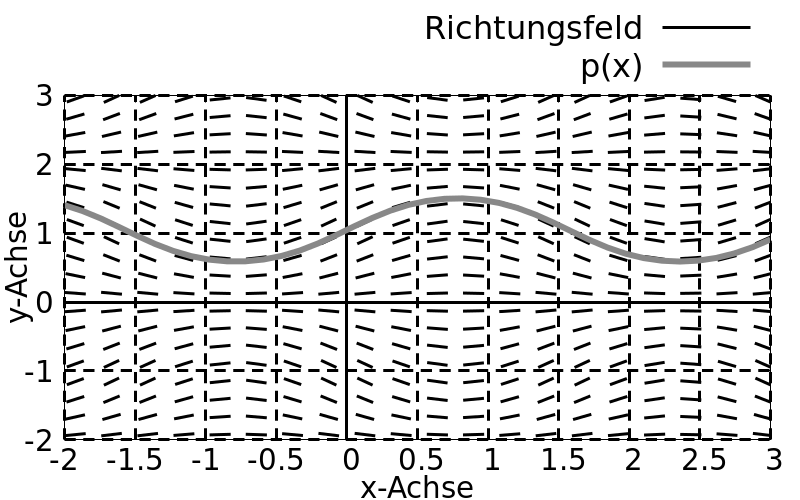
\includegraphics[width=0.95\textwidth]{grid-trial.png}
\end{center}

\begin{enumerate}[label=(\alph*)]
\item (3P) Definieren Sie anhand der Skizze den Begriff "Richtungsfeld" und erläutern Sie stichpunktartig den Unterschied zwischen "allgemeiner" und "partikulärer" Lösung.

\bigskip
\bigskip
\bigskip
\bigskip
\bigskip
\bigskip
\bigskip
\bigskip
\bigskip

\item (2P) Tragen Sie in die Skizze die Lösung des Anfangswertproblems $y(0) = \cos(180^\circ)$ ein!

\bigskip

\item (3P) Tragen Sie in die Skizze die grafische Bedeutung des Ausdrucks $\int\limits_1^2 p(x) \d{x}$ ein. Lesen Sie weiterhin die Koordinaten aller Punkte ab, an denen $p'(x)=0$ gilt!

\bigskip
Koodinaten der Punkte: 

\end {enumerate}

\newpage
\section* {Aufgabe 2} Mittels dem sogenannten "Newton'schen Verfahren" kann die Nullstelle einer Funktion $f(x)$ ermittelt werden. Dazu muss ein initialer Schätzwert $x_1$ für die Nullstelle gegeben sein. Es können dann schrittweise der Nullstelle näherkommende Schätzungen mittels der folgenden Zahlenfolge berechnet werden:

$$x_{n+1} = x_n - \frac{f(x_n)}{f'(x_n)}$$

\begin{enumerate}[label=(\alph*)]

\item (2P) Handelt es sich um die explizite oder rekursive Darstellung? (Begründung!)

\bigskip
\bigskip
\bigskip
\bigskip
\bigskip
\bigskip
\bigskip

\item (5P) Geben Sie die Rekursionsvorschrift für $f(x)=x^2-2$ an! Ermitteln Sie für $x_1=2$ die Glieder $x_2$ und $x_3$ als vollständig gekürzten Bruch!

\bigskip
\bigskip
\bigskip
\bigskip
\bigskip
\bigskip
\bigskip

\item (2P) Geben Sie den Grenzwert $\lim\limits_{n\to\infty}x_n$ für die in (b) gegebene Funktion $f$ an! (Hinweis: Aufgabentext oben genau lesen!)

\end{enumerate}

\newpage
\section* {Aufgabe 3}

Gesucht ist ein Näherungswert für $\zeta(2{,}1)$. Hierzu werde die Taylorentwicklung \textbf{2. Grads} der skalierten Zetafunktion $\zeta(x)$ an der \textbf{Entwicklungsstelle} {$\mathbf{x_0=2}$ betrachtet. Folgende Werte der Zetafunktion benötigen Sie möglicherweise:

\begin{center}
\begin{tabular}{ c | c | c | c | c}
 $\zeta(2)$ & $\zeta'(2)$ & $\zeta''(2)$ & $\zeta'''(2)$ & $\zeta'''(2{,}1)$ \\
 \hline
 1{,}00         &  -0{,}57         & 1{,}21           &  -3{,}65           & -2{,}49
\end{tabular}
\end{center}

\begin{enumerate}[label=(\alph*)]

\item (5P) Ermitteln Sie mit der Taylorentwicklung einen Näherungswert für $\zeta(2{,}1)$ auf 2 Kommastellen genau!

Taylorformel: $\sum\limits_{k=0}^n\frac{\zeta^{(k)}(x_0)}{k!}(x-x_0)^k$

\bigskip
\bigskip
\bigskip
\bigskip
\bigskip
\bigskip
\bigskip
\bigskip
\bigskip
\bigskip
\bigskip
\bigskip
\bigskip
\bigskip
\bigskip
\bigskip
\bigskip

\item (4P) Schätzen Sie den Fehler auf den in (a) ermittelten Wert  ab (Rundung auf die erste von null verschiedene Kommastelle)!\\
Hinweis: Für $x>1$ ist $\zeta'''(x)$ streng monoton steigend.

Restgliedabschätzung: $|R_n(x)| \le \frac{|x_0-x|^{n+1}}{(n+1)!}\cdot\max\limits_{\vartheta\in[x,x_0]} |f^{(n+1)}(\vartheta)|$


\end{enumerate}

\newpage
\section* {Aufgabe 4}

Es werde die DGL $y'''-2y''+y'=x$ betrachtet.

\begin{enumerate}[label=(\alph*)]

\item (3P) Klassifizieren Sie diese DGL bezüglich Ordnung, Linearität und Homogenität! 

\bigskip
\bigskip
\bigskip
\bigskip
\bigskip

\item (3P) Wie lautet die zugehörige homogene DGL? Erläutern Sie knapp, wie aus den Fundamentallösungen die allgemeine Lösung der homogenen DGL gefunden werden kann! Wie viele Fundamentallösungen sind für diese DGL notwendig?

\bigskip
\bigskip
\bigskip
\bigskip
\bigskip
\bigskip
\bigskip
\bigskip
\bigskip
\bigskip
\bigskip

\item (3P) Prüfen Sie, ob $y(x) = x^2+4x$ eine partikuläre Lösung der DGL darstellt!


\end{enumerate}

\label{LastTask}

\newpage

\begin{center}
{\bf {\large Musterlösung}}
\end{center}

\begin{center}
{\bf {\large Klausur Analysis (3IT19, 3MI19) - 13.02.2020}}
\end{center}

\begin{center}
\textbf{Jeder Anführungspunkt entspricht einem erteilten Bewertungspunkt.} 

Ist ein Rechenschritt falsch, werden für darauf basierende Rechnungen Punkte erteilt (Folgefehler), es sei denn, die Rechnung wird dadurch wesentlich vereinfacht. 
\end{center}

\begin{enumerate}

% Task 1
\item Jede verständliche Beschreibung wird akzeptiert. Folgende Formulierung ist nur ein Beispiel
\begin{enumerate}


\item
\begin{itemize}
\item Richtungsfeld gibt durch Liniensegmente den Anstieg der Funktion in jedem Punkt an.
\item Allgemeine Lösung ist die Kurvenschar (Menge) aller Lösungsfunktionen.
\item Partikuläre Lösung ist eine konkrete Funktion aus dieser Kurvenschar.
\end{itemize}

\item 
\begin{itemize}
\item Die eingetragen Funktion verläuft durch $(0,-1)$.
\item Der Funktionsgraph folgt etwa den eingezeichneten Richtungslinien.
\end{itemize}

\item $p(x) = \frac{1}{2}(x+1)(x-1)(x-2)$
\begin{itemize}
\item Fläche unter Graph von $p$ mit x-Achse zwische $x=1$ und $x=2$ ist markiert
\item Alle 3 Koordinaten, wo Ableitung 0 ist, wurden angegeben
\item Werte sind etwa korrekt: $(-0{,}75;0{,}50)$, $(0{,}75;1{,}50)$, $(2{,}4;0{,}50)$
\end{itemize}

\end{enumerate}

% Task 2

\item
\begin{enumerate}

\item
\begin{itemize}
\item Rekursiv.
\item Da Anfangswert $x_1$ und Berechnungsvorschrift für Folgeglied $x_{n+1}$ gegeben ist.
\end{itemize}

\item
\begin{itemize}
\item $f(x) = x^2-2$, $f'(x) = 2x$
\item $x_{n+1} = x_n - \frac{x_n^2-2}{2x_n}$
\item $x_2 = 2-(2^2-2)/4 = 2-2/4=\frac{3}{2}$
\item $x_3 = \frac{3}{2} - ((\frac{3}{2})^2-2)/3 = \frac{3}{2} - \frac{1}{12}$
\item $x_3 = \frac{17}{12}$
\end{itemize}

\item Da nicht genauer beschrieben: positive (eigentlich korrekte) und negative Lösung wird akzeptiert.
\begin{itemize}
\item Nach Aufgabenstellung konvergiert Zahlenfolgen gegen Nullstelle von $f$.
\item $x^2-2=0 \implies x=\pm\sqrt{2}$ ist also Grenzwert. 
\end{itemize}

\end{enumerate}


\newpage

% Task 3

\item
\begin{enumerate}

\item
\begin{itemize}
\item $\zeta(x) \approx \zeta(1{,}{00}) + \zeta'(2)(x-2) + \frac{1}{2}\zeta''(2)(x-2)^2$
\item $\zeta(x) \approx 1{,00} - 0{,}57(x-2) + 0{,}605(x-2)^2$
\item $\Gamma(2{,}1) \approx 1{,}00 - 0{,}57 / 10 + 0{,}605 / 100$
\item $= 1{,}00 - 0{,}057 + 0{,}000605$
\item $= 0{,}943605 \approx 0{,}94$
\end{itemize}

\item
\begin{itemize}
\item $|R_2(2{,}1)| \le \frac{0{,}1^3}{6}\cdot\max\limits_{\vartheta \in [2{,}0;2{,}1]} |\zeta'''(x)|$
\item Da $\zeta'''$ monoton steigend, ist Maximalwert $\zeta'''(2{,0}) = 3.65$ \\
      $|R_2(2{,}1)| \le \frac{0{,}1^3}{6}\cdot 3{,}65$
\item $ = 0{,}001\cdot 3{,}65/6$
\item $ = 0{,}68.../1000 \approx 0{,}0007$
\end{itemize}

\end{enumerate}

% Task 4

\item 
\begin{enumerate}

\item 
\begin{itemize}
\item Ordnung 3, da $y'''$ höchste Ableitung
\item Linear, da DGL Form der im Unterricht besprochenen allg. lin. DGL n-ter Ordnung hat
\item Inhomogen, da Homogenität auf rechter Seite $x\ne 0$ ist.
\end{itemize}

\item 
\begin{itemize}
\item Homogene DGL: $y'''-2y''+y' = 0$
\item Allgemeine Lösung ist Linearkombination der Fundamentallösungen
\item 3 Fundamentallösungen, da Ordnung 3
\end{itemize}

\item 
\begin{itemize}
\item $y'=2x+4$, $y''=2$, $y'''=0$
\item $y'''-2y''+y' = -4+2x+4 = 2x \ne x$
\item Unwahre Aussage, daher ist $x^2+4x$ keine Lösung der DGL
\end{itemize}

\end{enumerate}

\end{enumerate}


\end{document}
